
\section{Conjuntos abertos em $\mathbb R^n$}
\begin{definition}
    Um conjunto $U \subseteq \mathbb R^n$ é dito aberto se, para todo $x \in U$, existe um raio $r > 0$ tal que a bola aberta $B(x, r)$ está contida em $U$.
\end{definition}
\begin{proposition}
    Sobre abertos de $\mathbb R^n$, temos as seguintes propriedades.
    \begin{enumerate}
        \item $\mathbb R^n$ e o conjunto vazio $\emptyset$ são abertos.
        \item A união de qualquer coleção de conjuntos abertos é aberta.
        \item A interseção de dois conjuntos abertos é aberta.
        \item Bolas abertas são conjuntos abertos.
    \end{enumerate}
\end{proposition}
\begin{proof}
    É imediato que $\mathbb R^n$ e $\emptyset$ são abertos.

    Se $\mathcal C$ é uma coleção de conjuntos abertos, então $\bigcup \mathcal C=\bigcup_{U \in \mathcal C} U$ é aberto, pois, se $x \in \bigcup \mathcal C$, então existe $U \in \mathcal C$ tal que $x \in U$.
    Como $U$ é aberto, existe um raio $r > 0$ tal que $B(x, r) \subseteq U \subseteq \bigcup \mathcal C$.

    Se $U, V\subseteq \mathbb R^n$ são abertos, então $U\cap V$ é aberto, pois, se $x \in U\cap V$, então $x \in U$ e $x \in V$. Assim, existe um raio $r_1 > 0$ tal que $B(x, r_1) \subseteq U$, e um raio $r_2 > 0$ tal que $B(x, r_2) \subseteq V$. Tomando $r = \min\{r_1, r_2\}$, temos $B(x, r) \subseteq U\cap V$.

    Agora verifiquemos que bolas abertas são abertas.
    Considere uma bola aberta $B(p, r)$, onde $p \in \mathbb R^n$ e $r > 0$.
    Fixe $q \in B(p, r)$.
    Devemos ver que existe um raio $s > 0$ tal que $B(q, s) \subseteq B(p, r)$.
    Como $q \in B(p, r)$, temos $d(q, p) < r$.
    Assim, podemos tomar $s = r - d(q, p) > 0$.
    \begin{figure}
    \centering
    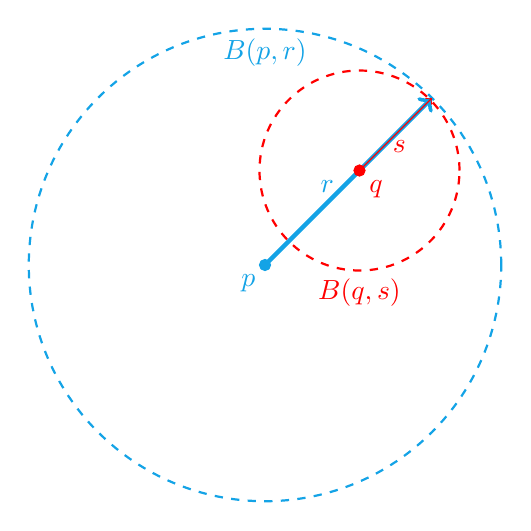
\begin{tikzpicture}
    % Bola B(p, r)
    \draw[thick, dashed, Cerulean] (0,0) circle (3);
    \filldraw[Cerulean] (0,0) circle (2pt) node[below left] {$p$};
    \node[Cerulean] at (0,2.7) {$B(p, r)$};
    % Raio r
    \draw[ultra thick,Cerulean,->] (0,0) -- (2.12,2.12);
    \node[Cerulean, left] at (1,1) {$r$};

    % Bola B(q, s)
    \filldraw[Red] (1.2,1.2) circle (2pt) node[below right] {$q$};
    \draw[thick, dashed, Red] (1.2,1.2) circle (1.27);
    \node[Red] at (1.2,-0.35) {$B(q, s)$};
    % Raio s
    \draw[Red,->] (1.2,1.2) -- (2.12,2.12);
    \node[Red, right] at (1.5,1.5) {$s$};

    % Relação de inclusão
    \end{tikzpicture}
    \caption{Relação de inclusão entre as bolas abertas.}
    \end{figure}
    O raio $s$ funciona: de $x \in B(q, s)$, temos que $d(x, q) < s$, e, portanto, $d(x, p)\leq d(x, q) + d(q, p) < s + d(q, p) =r$.

    Assim, $x \in B(p, r)$.
\end{proof}

Conjuntos abertos serão importantes ao trabalhar com diferenciabilidade.
\section{Curvas e diferenciabilidade de curvas}
\begin{definition}
Uma curva (contínua) em $\mathbb R^m$ é uma função contínua $f: I\rightarrow \mathbb R^m$, onde $I$ é um intervalo de $\mathbb R$.
\end{definition}

\begin{definition}
    Seja $I\subseteq \mathbb R$ um conjunto aberto e $f: I\rightarrow \mathbb R^m$ uma função contínua.

    Para $s \in I$, dizemos que $f$ é \emph{diferenciável}, ou \emph{derivável} em $s$ se existir o limite a seguir:

    \begin{equation}\label{eq:derivada}
        \lim_{t \to s} \frac{f(s)-f(t)}{s-t}
    \end{equation}

    Caso $f$ seja diferenciável em $s$, denotamos tal limite por $f'(s)$, e o chamamos de derivada de $f$ em $s$.

    Se $f$ é diferenciável (derivável) em todos os pontos de $I$, dizemos que $f$ é \emph{diferenciável (derivável)}.
\end{definition}

Observação: o limite na equação \eqref{eq:derivada} é o limite da função $g$ cujo domínio é $I\setminus \{s\}$ e dada por $g(t) = \frac{f(s)-f(t)}{s-t}$.

O ponto $s$ é um ponto de acumulação de $I\setminus\{s\}$, pois, se fosse isolado, existiria $\delta>0$ tal que $B(s, \delta)\cap I\setminus\{s\}=\emptyset$.
Ao mesmo tempo, $I$ é aberto, logo, encolhendo $\delta$ se necessário, podemos garantir que $B(s, \delta)\subseteq I$.
Mas $B(s, \delta)$ possui outros pontos além de $s$, o que é absurdo.

\begin{proposition}
    Seja $I\subseteq \mathbb R$ um conjunto aberto e $f: I\rightarrow \mathbb R^m$.

    Seja $s \in I$.
    
    Então $f$ é derivável em $s$ se, e somente se, cada função coordenada $f_i$ é derivável em $s$.
    Nesse caso, temos que $f'(s) = (f_1'(s), \dots, f_m'(s))$.
\end{proposition}
\begin{proof}
    Primeiro, suponha que $f$ é derivável em $s$.

    Temos que existe o limite $f'(t)$ de $g$ em $s$, onde $g(t) = \frac{f(s)-f(t)}{s-t}$.

    Temos que a $i$-ésima coordenada de $g$ é dada por $g_i(t) = \frac{f_i(s)-f_i(t)}{s-t}$.
    Logo, a $i$-ésima coordenada de $f'(s)$ é o limite de $g_i$ em $s$. Porém, por definição, também é $f_i'(s)$.

    Assim, concluímos que $f'(s) = (f_1'(s), \dots, f_m'(s))$.

    Reciprocamente, suponha que cada função coordenada $f_i$ é derivável em $s$.

    Temos que, para cada $i$, $f_i'(s)$ é o limite de $g_i$ em $s$, e, portanto, existe o limite de $g$ em $s$, e este é dado por $(f_1'(s), \dots, f_m'(s))$.
\end{proof}

Funções deriváveis possuem o que chamamos de retas tangentes.
\begin{definition}
    Seja $I\subseteq \mathbb R$ um conjunto aberto, $a \in I$ e $f: I\rightarrow \mathbb R^m$ uma função derivável em $a$ tal que $f'(a)\neq 0$.

    A reta tangente à trajetória (ou imagem) de $f$ em $a$ é a reta que passa por $f(a)$ e tem direção dada por $f'(a)$, ou seja, é o conjunto $r$ dado por:

    \begin{equation*}
        \{f(a) + t f'(a) : t \in \mathbb R\}.
    \end{equation*}

    Nesse caso, dizemos que $r$ é \emph{uma} reta tangente à trajetória de $f$ em $a$.
\end{definition}

Além disso, temos a melhor aproximação linear possível para $f$ em $a$.
\begin{definition}
    Seja $I\subseteq \mathbb R$ um conjunto aberto, $a \in I$ e $f: I\rightarrow \mathbb R^m$ uma função derivável em $a$.

    A \emph{melhor aproximação linear de $f$ em $a$} é a função $T: \mathbb R \to \mathbb R^m$ dada por:
    \begin{equation*}
        T(t) = f(a) + (t-a)f'(a).
    \end{equation*}
\end{definition}

\begin{proposition}
    Seja $I\subseteq \mathbb R$ um conjunto aberto, $a \in I$ e $f: I\rightarrow \mathbb R^m$.

    Se $f$ é derivável em $a$, então a melhor aproximação de $f$ em $a$, $T: \mathbb R \to \mathbb R^m$, é a única função afim (ou seja, a única função da forma $T(t) = w + t v$, onde $w, v \in \mathbb R^m$) tal que:
\begin{enumerate}[label=(\alph*)]
    \item $T(a)=f(a)$, e
    \item $\lim_{t \to a} \frac{f(t)-T(t)}{|t-a|} = 0$.
\end{enumerate}
    Reciprocamente, $f$ admite uma função $T: \mathbb R \rightarrow \mathbb R^n$ afim que satisfaz (a) e (b), então $f$ é derivável em $a$ e $T$ é a melhor aproximação linear de $f$ em $a$.
\end{proposition}
\begin{proof}
    Para a primeira parte, primeiro note que $T(a) = f(a) + (a-a)f'(a) = f(a)$.

    Agora, vejamos que $\lim_{t \to a} \frac{f(t)-T(t)}{|t-a|} = 0$.
    De fato, temos:
    \begin{align*}
        \lim_{t \to a} \frac{f(t)-T(t)}{|t-a|} &= \lim_{t \to a} \frac{f(t)-f(a)-(t-a)f'(a)}{|t-a|} \\
        &= \lim_{t \to a} \frac{f(t)-f(a)}{t-a}-f'(a) \\
        &= 0,
    \end{align*}
    pois $f'(a)$ é o limite de $\frac{f(t)-f(a)}{t-a}$ em $a$.

    Para o resto da proposição, seja $T(t) = w + t v$ uma função afim que satisfaz (a) e (b).
    Veremos que $f$ é derivável e que $T$ é a melhor aproximação linear de $f$ em $a$.

    Primeiro, por $a$, temos que $w + a v = f(a)$, ou seja, $w = f(a) - a v$.
    Assim, $T(t) = f(a) + (t-a)v$.

    Por (b), temos que:
    \begin{align*}
        0 &= \lim_{t \to a} \frac{f(t)-T(t)}{|t-a|} \\
        &= \lim_{t \to a} \frac{f(t)-f(a)-(t-a)v}{|t-a|} \\
        &= \lim_{t \to a} \frac{f(t)-f(a)}{t-a}-v.
    \end{align*}

    Logo:
    \begin{equation*}
        v = \lim_{t \to a} \frac{f(t)-f(a)}{t-a}
    \end{equation*}
    e, portanto, $f$ é derivável em $a$ e $f'(a) = v$.
    Assim, $T$ é, por definição a melhor aproximação linear de $f$ em $a$.
\end{proof}
